\documentclass[conference]{IEEEtran}
\IEEEoverridecommandlockouts
% The preceding line is only needed to identify funding in the first footnote. If that is unneeded, please comment it out.
%Template version as of 6/27/2024

\usepackage{cite}
\usepackage{amsmath,amssymb,amsfonts,amsthm}
\usepackage{algorithmic}
\usepackage{graphicx}
\usepackage{textcomp}
\usepackage{xcolor}
\usepackage{hyperref}
\def\BibTeX{{\rm B\kern-.05em{\sc i\kern-.025em b}\kern-.08em
    T\kern-.1667em\lower.7ex\hbox{E}\kern-.125emX}}
\newtheorem{definition}{Definition}
\newtheorem{theorem}{Theorem}
\newtheorem{lemma}{Lemma}
\newcommand{\qm}[1]{``#1"}
\usepackage{mathtools} % for 'dcases*' env.


%\onecolumn
%
%\title{Relations between Causality, Fairness, Privacy, Accuracy, Information Flow and Explainability in Machine Learning\large\\ Type: Scientific\\Advisor: Mário Sérgio Alvim}
%\author{Artur Gaspar da Silva}
%\date{16/01/2025}
%
%
\begin{document}
%
%
%\begin{titlepage}
%    \begin{center}
%
%        \Huge
%        \textbf{Universidade Federal de Minas Gerais}
%
%        \vspace{0.5cm}
%        \LARGE
%            Department of Computer Science
%
%        \vspace{0.5cm}
%        \large
%           Undergraduate Thesis, Part II 
%
%        \vspace{0.7cm}
%
%        
\includegraphics[width=0.4\textwidth]{logoUFMG.jpg}
%
%
%
%        \vspace{0.5cm}
%
%        \Huge
%            Relations between Fairness, Privacy and Quantitative Information Flow in Machine Learning
%            \\\large Type: Scientific
%
%        \vspace{0.5cm}
%        \begin{abstract}
%            Recent years have witnessed an enormous advance in the area of Machine Learning, reflected by the popularity of Artificial Inteligence systems. For most of the history of machine learning research, the main goal was the development of machine learning algorithms that led to more accurate models, but it is now very clear that there are many other important areas to develop. We want models to be fair to unprivileged groups in society, to not reveal private information used in the model training, to provide comprehensible explanations to humans in order to help identifying causal relationships, among many relevant goals other than simply improving model accuracy. In this work, we explore possible new relationships between fairness, privacy and Quantitative Inforamtion Flow. The first exploration is an analysis of papers that explore the impact of privacy-enhancing mechanisms on Machine Learning fairness notions. Our second exploration is the possibility of dividing a fixed local differencial privacy budget between variables with varying degrees of sensitivity. Finally, we explore modeling both local differential privacy parameters within the Quantitative Information Flow framework.
%        \end{abstract}
%
%        \vspace{0.5cm}
%
%
%     \end{center}
%
%\raggedright
%
%\Large
%    Supervisor:
%    \vspace{0.2cm}\\
%\Large
%    Prof. Mário Sérgio Alvim
%    \vspace{0.125cm}\\
%
%\raggedleft
%
%\Large
%    Thesis written by:
%    \vspace{0.125cm}\\
%\Large
%    Artur Gaspar da Silva
%
%
%
%\begin{center}
%    \vspace{1cm}
%        Academic Semester 2024/2
%\end{center}
%
%\end{titlepage}
%%\maketitle
%
%
%\newpage
%\tableofcontents
%\begin{IEEEkeywords}
%    Quantitative Information Flow, Differential Privacy, Fairness, Machine Learning.
%\end{IEEEkeywords}
%\newpage
%\twocolumn



\title{Relations between Fairness, Privacy and Quantitative Information Flow in Machine Learning
            \\\large Type: Scientific\\Advisor: Mário Sérgio Alvim

}

\author{\IEEEauthorblockN{1\textsuperscript{st} Artur Gaspar da Silva}
\IEEEauthorblockA{\textit{Departamento de Ciencia da Computaçãp (DCC)} \\
\textit{Universidade Federal de Minas Gerais (UFMG)}\\
Belo Horizonte, Brazil \\
artur.gaspar@dcc.ufmg.br}
}

\maketitle

\begin{abstract}
            Recent years have witnessed an enormous advance in the area of Machine Learning, reflected by the popularity of Artificial Inteligence systems. For most of the history of machine learning research, the main goal was the development of machine learning algorithms that led to more accurate models, but it is now very clear that there are many other important areas to develop. We want models to be fair to unprivileged groups in society, to not reveal private information used in the model training, to provide comprehensible explanations to humans in order to help identifying causal relationships, among many relevant goals other than simply improving model accuracy. In this work, we explore possible new relationships between fairness, privacy and Quantitative Inforamtion Flow. The first exploration is an analysis of papers that explore the impact of privacy-enhancing mechanisms on Machine Learning fairness notions. Our second exploration is the possibility of dividing a fixed local differencial privacy budget between variables with varying degrees of sensitivity. Finally, we explore modeling both local differential privacy parameters within the Quantitative Information Flow framework.
\end{abstract}

\begin{IEEEkeywords}
Quantitative Information Flow, Differential Privacy, Fairness, Machine Learning.
\end{IEEEkeywords}




\section{Introduction}
Recent resarch \cite{Sok}\cite{Reductions}\cite{Rachel}\cite{Awareness} indicates numerous tensions and synergies between many concepts that surround the Machine Learning literature, including Fairness, Privacy, Accuracy and Interpretability. For instance, there is an inherent tradeoff between Fairness and Accuracy such that, depending on the data distribution, it might be impossible to develop a model that achieves acceptable values for both fairness and accuracy, if we considr some reasonable fairness metrics \cite{Carlos}. Also, there has been some work on introducing Causality concepts into the discussion, for instance, to develop better fairness metrics \cite{CausalFair}. It has also been suggested to use interpretable models (as explanations to more complex models) for auditing systems and checking if they are fair, although this might lead to problems \cite{ExplainAll}. This area of research is especially relevant nowadays, given the importance that Machine Learning and Artificial Intelligence systems have: we now have computational systems that are part of processes of making decisions with big impacts on people's lives, for instance, recidivism prediction \cite{Compass}, loan approvals \cite{Loans}, hiring decisions \cite{Jobs}, and others.

The goal of this Undergraduate Thesis is to review and reproduce results presented in the litearture, verify the viability of the connections between the aforementioned areas and Quantitative Information Flow, and, if possible, develop new theoretical results. This project is divided into two parts: POC I and POC II. In POC I, the specific goals were to research the literature for these concepts and focus on the connections that have been identified between them, so the expected result is a concise review of the literature on these topics. In this work (POC II), we verify possible connections between Privacy, Fairness and Quantitative Information Flow, and outline possible new theoretical results. We provide an in-depth theoretical analysis of the viability of Quantitative Information Flow approaches to these areas and the connections between privacy and fairness. We provide a formal exploration of the impact of privacy-enhancing obfuscation methods in fairness, based on important results in the literature reviewed in POC I, we explore how the privacy budget can be divided between many variables in the context of Local Differential Privacy, and, finally, we explore how viable is the application of the Quantitative Information Flow framework in Local Differential Privacy.

\section{Theoretical Reference}

Fairness in Machine Learning is concerned with measuring how unfair the results provided by Machine Learning models are to certain groups or individuals \cite{FairMeasures}, and improving how fair the models are \cite{FairSolve}. There are tensions between different fairness measures \cite{Impossibility}\cite{FairTensions}. Privacy is concerned with quantifying how much sensitive information leaks about individuals and methods to avoid this information leakage. In Machine Learning settings, the data collection might be hard for information that is considered very sensitive (for instance, whether or not a person regularly uses illegal drugs) and approaches such as Differential Privacy \cite{DP} might improve trust in the data collection. Also, the model itself might allow the identification of individuals and sensitive features, which is not desirable \cite{liu2021machine}. Quantitative Information Flow is a general theoretical framework for measuring amounts of information, with a focus on privacy applications but, in principle, a broader scope \cite{QIF}. In recent research \cite{Sok}, the relationships between Fairness, Interpretability and Privacy have been extensively explored. Recent papers focuses on relationships between Privacy and Fairness \cite{Awareness}, on the relationship between Privacy \cite{Rachel}, and on the feasibility regions of Accuracy and Fairness metrics \cite{Carlos}\cite{Reductions}. 

More specifically to the relation between Differential Privacy and Quantitative Inforamtion Flow, there are important results in the literature. There are works discussing the relations between differential privacy and $g$-vulnerability, including bounds on $g$-leakage as a function of the $\epsilon$ parameter of differential privacy, and the fact that there is no bound on differential privacy as a function of the $g$-vulnerability \cite{alvim2015information}. Also, we have recent work \cite{fernandes2022explaining} discussing how the $\epsilon$ parameter of Differential Privacy is related to max-case $g$-vulnerability: $e^\epsilon$ is exactly the multiplicative max-case channel capacity under a fixed prior. This work also discusses many other theoretical results relating $g$-vulnerability notions with differential privacy. 

\subsection{Machine Learning and scenario considered}

Machine Learning is the field of study that focuses on developing methods of learning general patterns from limited data. In recent years, important advances have been observed in Machine Learning research, and also the popularity and applications of some methods have increased significantly. One example is the improvement of Convolutional Neural Network architectures, and the popularity of Generative Models. Also, some recent research is focused on the theory behind such machine learning methods \cite{SAAMAP}\cite{grohs2022mathematical}, and statistical learning in general \cite{Vapnik}. Part of the goal of this formalization is to provide more qualitative guarantees in regard not only to accuracy, but also fairness, privacy, interpretability, and other important qualities. We discuss some of these different goals in the next two subsections.

In general, we consider \emph{supervised learning} problems: in this scenario, a \emph{machine learning algorithm} is an algorithm that receives many data points, which we call \emph{training data}, and outputs a \emph{model}. This model is itself an algorithm that receives a data point with some information omitted, encoded in what we call the \emph{target variable}, and outputs a guess of the omitted information, which we call the \emph{model prediction}. The model is then evaluated with other data points, ideally not the same ones used for training the model. This is called supervised learning because the algorithm has access to the target variable during the training process, which is not the case for unsupervised learning.

Figure \ref{fig:EEAAO} shows how the other concepts are related to machine learning in this context: we usually can assume that the training data is generated by some causal process, which can be modeled by a causal model; possible privacy attacks include performing sensitive information inference on the training data and on the model itself; we usually measure how accurate and fair a system is by analyzing its predictions for many data points; we can also obtain local and global explanations for complex models by this type of analysis. Throughout this wor, we focus on privacy and fairness, and how these concepts might be modeled within the Quantitative Information Flow framework.

\begin{figure*}[ht]
\centering
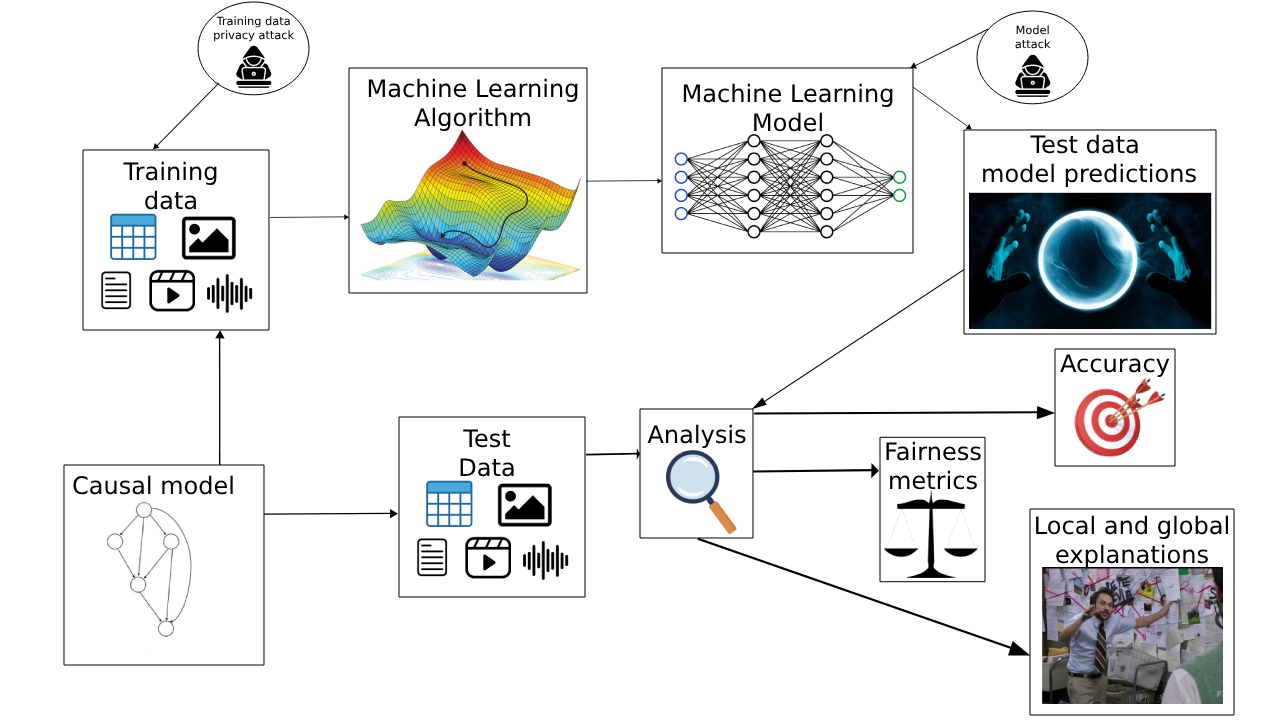
\includegraphics[width=\textwidth]{EverythingEAAO}
\caption{Figure representing the supervised learning scenario we consider throughout this work, with a focus on privacy and fairness.}\label{fig:EEAAO}
\end{figure*}

\subsection{Fairness}

In the context of Machine Learning, fairness refers to the reduction, as much as possible, of \emph{algorithmic bias}, the bias introduced by algorithmic decisions. This bias might have a big social impact because this can expand existing unfair discrimination in society, as machine learning algorithms are being used to make more and more important decisions. One famous example is the COMPAS recidivism algorithm, which has been used by the United States courts to estimate how likely someone is to reoffend in the future. It was revealed \cite{Compass} that this tool was heavily biased against black people. 

For binary classification, we will say that the result is \emph{positive} for a data point if it benefits the person represented by that data point, and \emph{negative} otherwise. We will say that the \emph{unprivileged group} is the group of people affected negatively by the bias, and the \emph{privileged group} is the other group of people.

Such biases can happen because of many factors. The algorithm itself might introduce bias, or the data might be biased. The data may have been collected in a biased way (in the COMPAS example, this would be the case if reincidivism data was collected more for black reincidivists than for white), or the data might be simply reinforcing some bias in society. 

Also, the bias in society might be such that the data is in disagreement with reality (the unprivileged group's true values for the target variable would affect them in the same way as the privileged group), or it is in agreement with reality because of structural biases in society. For instance, if the prediction of the algorithm is whether someone will have good grades if accepted to some university, people in the unprivileged group might not have had as good oportunities in life as people in the privileged group, so the data is correct when it says that those people will have worse grades. Even so, the results might still be considered unfair, as this depends on the notion of fairness we consider. All of these unfairness scenarios can be further divided into other types of unfairness, as was done in previous works \cite{mehrabi2021survey}. Image \ref{fig:whereUnfair} illustrates where unfairness might come from, and we summarize below the ways in which unfairness might be introduced:

\begin{enumerate}
\item Algorithm results do not reflect the data.
    \begin{enumerate}
    \item The algorithm might optimize for the majority only, achieving good overall accuracy even though it's mostly wrong for minorities. This can be considered a type of Aggregation Bias.
    \item Systematic errors in the algorithm, that lead to biased estimation.
    \end{enumerate}
\item The data can be biased, not reflecting the reality.
    \begin{enumerate}
    \item We can have structural biases in society, such that people in unprivileged groups do not have the necessary opportunities, but if they were treated similarly to the privileged group by society, they would have similar results. For instance, an unprivileged group that doesn't have good educational opportunities will have worse scores on exams because of historical discrimination, and although just looking at whether someone is in this group could lead to a good accuracy, it might only perpetuate current unfair biases in society.
    \item The bias can also be introduced in a way that people in the unprivileged group were misclassified before the data was collected. For instance, maybe capable people in an unprivileged group usually don't get a job even though they are actually as capable as the unprivileged group.
    \item Data collection doesn't reflect the reality: Measurement bias (for instance, COMPASS used friend/family arrests as a proxy for a risk score present in the dataset), Omitted Variable Bias (this violates assumptions of some learning models, for instance linear regression models usually assumes error terms uncorrelated with the parameters considered in the regression), Representation/Sampling Bias (biased sampling lacking the diversity of the population), Simpson's Paradox (if we don't have data on a confounder, correlations might be spurious \cite{Causality}).
    \item If the data is collected on a group fundamentally distinct from the one where it will be used, for instance another population (Population Bias) or the same population but at another time (Temporal Bias), unfair bias might be introduced.
    \item Data that relies on people's opinion is prone to many biases: Social Bias (people do what others are doing), Self-Selection Bias (people think that everyone agrees with them), and many others.
    \end{enumerate}
\item Data might depend on the algorithm's previous output: Presentation Bias (the user is presented to some selected advertisements, for instance), Ranking Bias (search engines ordering results in a biased way), Popularity Bias (more popular items are shown more). This might strengthen biases through time. 
\item Finally, the circumstances can change through time, either by the influence of the algorithm itself or other factors, which can worsen the quality of algorithms previously considered able to provide good results (Emergent Bias).
\end{enumerate}



\begin{figure}[ht]
\centering
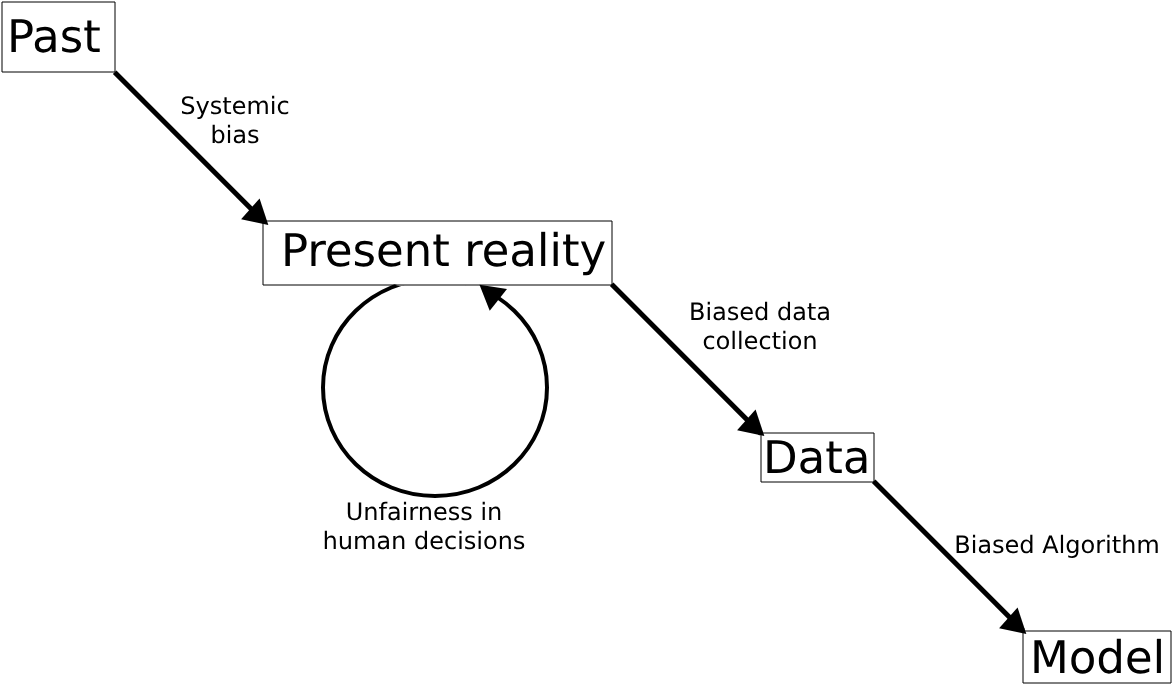
\includegraphics[width=\columnwidth]{whereUnfair}
\caption{Figure representing some of the main possible sources of unfairness.}\label{fig:whereUnfair}
\end{figure}

Besides biased data and deliberate bias in the algorithm, such that the results of the algorithm do not reflect the data, it is also possible to introduce bias because the algorithm might prioritize making correct predictions for the majority of the population, if it can't make correct predictions for both the majority and the minority. Another possibility is that the prediction might depend on past decisions of the algorithm, and we only know the result if the result provided is positive (for instance, we only know if someone will reincide if we release them). In this type of scenario, according to Learning Theory, it's important to take suboptimal decisions to \emph{explore} different options and gather more data \cite{chouldechova2018frontiers} (found in \url{arxiv.org}), which might be considered unethical as it might have a big cost to society (releasing someone that's probably going to commit more crimes) or to the individual (not giving a life-saving drug to some patients as an experiment to see the survival rates for that specific group). 

Many different notions of algorithmic fairness have been developed, and some are not compatible \cite{alves2023survey}. Initially, the notions of fairness could be grouped into two main types: statistical and individual definitions of fairness \cite{chouldechova2018frontiers}. Statistical (group) notions of fairness require some statistical metrics to be similar for certain demographic groups, and individual notions enforce constraints on pairs of individuals, for instance requiring similar individuals to be treated similarly. Many problems with statistical notions and why they, in general, don't provide good individual guarantees are presented in previous works \cite{Awareness}\cite{kearns2018preventing}. For instance, one such problem is satisfying the constraints for two protected attributes individually but not for combinations of these attributes. One problem with both individual and group notions is \emph{composition}: it is not always the case that satisfying fairness constraints in individual, isolated, components of a system imply that fairness constraints will be satisfied for the whole system \cite{dwork2018fairness}. Finally, there are also causal approaches to fairness notions. In general, it is not possible to satisfy some of the main notions of fairness at the same time \cite{hellman2020measuring}\cite{bell2023possibility}\cite{zemel2013learning}, and which fairness notion to use depends a lot on the specific goals of each different system.

We will now define some of the main notions of fairness, which are the ones we will consider in Subsection \ref{subsec:ldpunfair}. We consider that $Y$ is the binary target variable, with $Y=1$ as the positive result and $Y=0$ as the negative one; $A$ is the binary sensitive attribute, with $A=1$ for the privileged group and $A=0$ for the unprivileged group; $\hat Y$ is the model prediction of the target variable value; $X$ is a set of legitimate factors that can be used for classification.

\begin{definition}[Equal Opportunity Difference] We define \emph{Equal Opportunity Difference} as $P(\hat Y = 1| A = 1, Y =1) - P(\hat Y = 1| A = 0, Y = 1)$. Equal Opportunity is \emph{satisfied} if the Equal Opportunity Difference is equal to zero.
\end{definition}

\begin{definition}[Statistical Disparity] We define \emph{Statistical Disparity}, also known as \emph{Demographic Disparity}, as $P(\hat Y = 1| A = 1) - P(\hat Y = 1| A = 0)$. Statistical (Demographical) \emph{Parity} is \emph{satisfied} if the Statistical Disparity is equal to zero.
\end{definition}

\begin{definition}[Conditional Statistical Disparity] We define \emph{Conditional Statistical Disparity}, conditioned on $x$, as $P(\hat Y = 1| A = 1, X = x) - P(\hat Y = 1| A = 0, X = x)$. Conditional Statistical \emph{Parity} is \emph{satisfied} if the Conditional Statistical Disparity is equal to zero.
\end{definition}

A possible general definition of \emph{individual fairness} notions is that an algorithm is considered fair if it gives similar outcomes to similar individuals, according to similarity notions relevant to the specific scenario considered.

The techniques developed to reduce unfairness in algorithmic decision-making can be divided into \emph{pre-processing}, \emph{in-processing} and \emph{post-processing}. Pre-processing techniques modify the training data to remove biases present there. In-processing techniques modify the learning algorithm itself, for instance, by changing the objective learning function to include not only accuracy but also adding to it some statistical fairness metric, or including some constraint that it has to satisfy. Post-processing techniques act after the model is trained to reduce the unfairness in the decisions made by such a model.

In general, just removing the variables that would be considered unfair to use directly to classify an individual is not enough to guarantee fairness. As illustrated in image \ref{fig:correlated}, the variables we would remove might be highly correlated to other variables, which could be used by the model to discriminate almost as if we hadn't removed any variable. Also, even if the machine learning model itself didn't use any sensitive variables or correlated attributes for the predictions, we still need to collect this sensitive data to be able to measure how unfair the model is.

\begin{figure}[ht]
\centering
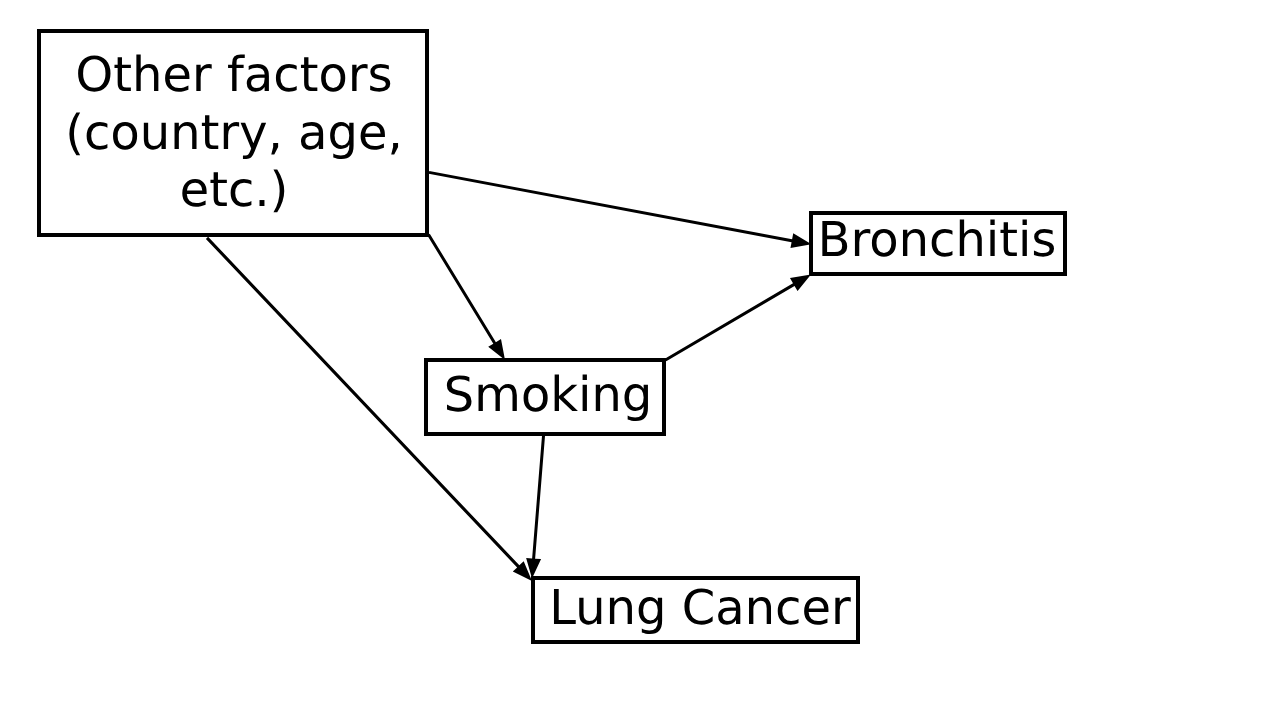
\includegraphics[width=\columnwidth]{correlated}
\caption{Figure representing potential correlations between sensitive variables and other factors: if the disease status is a sensible information that could be used for unfair discrimination, then removing this information might not be enough to avoid unfair discrimination, as smoking, age and other factors combined might lead to unfair discrimination almost as if the model had direct access to the sensitive values.}\label{fig:correlated}
\end{figure}


\subsection{Privacy}

In the context of Machine Learning, a privacy-preserving algorithm is one that does not allow information considered private/sensitive to be obtained by unauthorized parties. According to the terminology presented in \cite{liu2021machine}, this is called \emph{private ML}. The private information to be protected can be the data used to train the model or the model parameters and structure itself. It is also possible to use Machine Learning to enhance privacy, \emph{ML enhanced Privacy Protection}, or to serve as an attack tool, \emph{ML-based Privacy Attack}. We will focus on private ML.

We call \emph{adversary} the agent that wants to discover the private information, and \emph{secret} the private information itself. There are some possible goals of the adversary: she might wish to recover the model itself by trying to approximate the function that represents the model, to recover some feature or statistical property of the dataset, to discover whether some individual data point is present in the dataset, or even recover the exact values of individual samples in the dataset. We distinguish between the \emph{White-Box access} and \emph{Black-Box access} scenarios as the situation in which the adversary has or does not have full access to the trained model and their parameters, respectively. 

\emph{Model Extraction Attacks} assume an adversary with black-box access to the model, and no prior knowledge of the model parameters and training data. Some approaches to model extraction are presented in previous works \cite{tramer2016stealing}. Although the most efficient attacks rely on confidence values, attacks that rely only on the output class labels are also presented. Other works focused on estimating hyperparameters \cite{wang2018stealing} for an adversary that knows the training dataset and the Machine Learning algorithm. Notice that recovering the model can help in the development of attacks against the training data, even if the adversary doesn't have prior knowledge of the model.

\emph{Feature estimation attacks} focus on recovering statistical properties or features of the training dataset, for an adversary that does not know the training data or the its distribution. Some attacks are presented in previous works \cite{fredrikson2015model} both for black-box and white-box model access. As expected, the white-box attacks lead to better attacks, and they provide examples for recovering individual sensitive information from marital happiness answers in two different datasets and white-box attacks for recovering images in a face recognition model. The results lead to the possibility of (almost) identifying someone with only their name and the face recognition model and to the possibility of identifying the answer to a sensitive topic on a supposedly anonymous questionnaire (whether the person answering ever cheated on their significant other) with very high precision and a recall bigger than 20\%. 

The attacks presented in some previous works \cite{ateniese2015hacking} aims to recover statistical information about the training dataset by the use of many models trained on different datasets and a meta-classifier that identifies if a given model was trained in a dataset with some desired statistical property. This is a white-box scenario, and they focused on attacking Support Vector Machines and Hidden Markov Models. Another common type of attack is the Membership Inference Attack, reviewed in previous works \cite{hu2022membership}, in which the adversary aims to infer whether a given data point was used to train a given model or not. One approach is presented in a previous work \cite{carlini2022membership}, in which the adversary can sample from the original data distribution and has black-box access to the target model. It works by training many \qm{shadow models} by using the data distribution, half with the target data point and half without it, then performing some computations based on confidence scores to estimate how likely the real model is to have used the relevant data point.

We will now focus on methods of modeling the protection of training data from privacy attacks. The main methods we will mention are Differential Privacy, Local Differential Privacy, and Homomorphic Encryption. Local Differential Privacy will be the method we focus on in Subsections \ref{subsec:ldpunfair}, \ref{subsec:ldeltap} and \ref{subsec:ldeltap}.

\emph{Differential Privacy} (DP) is one of the most important definitions of quantifying privacy: the idea of DP is to define how hard it should be to distinguish one dataset from another that differs by at most any one individual data point. More generally, we can define how hard it should be to distinguish an element from a neighboring element, such that in the database example, the elements are databases and the neighboring relation is such that two databases are neighbors if and only if they differ by at most one data point. A (possibly randomized) algorithm that aims to obtain a dataset that is protected according to the DP definition is called a \emph{Differential Privacy Mechanism}. The formal definition is presented below. 

\begin{definition}[$\epsilon$-Differential Privacy]\label{def:epsilonLDP} A randomized algorithm from $\mathcal{X}$ to $\mathcal{Z}$ satisfies $\epsilon$-Differential Privacy, for $\epsilon > 0$, if for every $x,x' \in \mathcal{X}$ such that $x$ is a neighgboring element of $x'$, and for every $S \subseteq \mathcal{Z}$:
$$P(\mathcal{K}(x) \in S) \leq e^\epsilon P(\mathcal{K}(x')\in S)$$
\end{definition}

The parameter $\epsilon$ can be interpreted as how close we require the probabilities of neighboring datasets to be, such that smaller values of $\epsilon$ lead to stronger requirements. In some practical applications, the Differential Privacy restriction is too strong. Thus, we have a relaxed definition for Differential Privacy, in which the parameter $\delta$ can be interpreted as the probability that the DP guarantee will not be satisfied.:

\begin{definition}[$(\epsilon,\delta)$-Differential Privacy] A randomized algorithm from $\mathcal{X}$ to $\mathcal{Z}$ satisfies $(\epsilon,\delta)$-Differential Privacy, for $\epsilon > 0$ and $\delta \in [0,1]$, if for every $x,x' \in \mathcal{X}$ such that $x$ is a neighgboring element of $x'$.
$$P(\mathcal{K}(x) \in S) \leq e^\epsilon P(\mathcal{K}(x')\in S)+\delta$$
\end{definition}

\emph{Local Differential Privacy} (LDP) is a concept important when the data collector is not assumed to be trusted and consists of the same restrictions as Differential Privacy, but with $\mathcal{X}$ as the set of possible individual values, $\mathcal{Z}=\mathcal{X}$ and the neighboring relation being such that all possible values are neighbors. This algorithm should be applied locally by the owner of each data point.

The idea is that individuals apply noise locally in a way such that the data collector can still obtain the desired results with the noisy data. The classical example is the scenario in which we want to discover how many people do some illegal activity (for instance, use illegal drugs) in a given region. The person answering might be tempted to lie to not let this sensitive information leak. But if we tell them to toss two coins, such that if the first one comes up heads, they answer truthfully, but if not, then the answer should be \qm{yes} if the second coin came up heads and \qm{no} otherwise. We will know that approximately $\frac{1}{2}$ of the answers is not the true answer of the person, such that half of these are \qm{yes} and half \qm{no}. We can then remove $25\%$ of the total number of answers from the number of \qm{yes} and another $25\%$ from the total number of \qm{no} to estimate the real distribution. Previous works \cite{xiong2020comprehensive} delves into many mechanisms, information metrics, and applications relevant to Local Differential Privacy, including machine learning on private data.

There are some common misconceptions about what exactly are the assumptions of Local Differential Privacy. Notice, for instance, that if the data points of two individuals are known to be highly correlated (for instance, genetic data for two siblings), then even if their data points after the application of the LDP mechanism do satisfy $(\delta,\epsilon)$-LDP, the tuple of these two data points may not satisfy $(\delta,\epsilon)$-LDP, which can improve the inferences that an adversary can make. Imagine the extreme case: if we know that all data points are equal and the LDP mechanism gives a higher probability of not changing the data point, then the adversary can discover the common value of all data points simply by looking at the most common value after the mechanism is applied. This can also be a problem for Differential Privacy, as shown in previous works \cite{liu2016dependence}. 

The possible dependencies among data points have led to some different definitions of what exactly are the assumptions of LDP, for instance, that all data points are independent, or that the adversary knows all data points but one. Previous works \cite{tschantz2020sok} discuss how a causal interpretation can help in uncovering the meaning of each LDP assumption, which are or not equivalent, and also compares with potential causal notions of LDP.

\emph{Federated Learning} is another method that can help improve the privacy of individuals. The idea is that each individual trains a Machine Learning model locally, and shares information with a centralized server to improve a global model. The privacy risks are reduced because no individual data point and no individual user updates to the model are stored in the server. But still, without extra preparations, it might be possible to attack individual data points, as explored in previous works \cite{wang2019beyond}.

Finally, \emph{Homomorphic Encryption} is a form of encryption that allows computations to be done without decrypting the data, just the result is decrypted. \emph{Secure Multi-Party Computation} is also an option if there are multiple parties responsible for this computation. The major drawback of these methods is the significant additional computational cost. Homomorphic Encryption and Secure Multi-Party Computation have been proposed for frequency estimation \cite{yang2005privacy}, Deep Learning \cite{hesamifard2017cryptodl}\cite{goswami2024privacy}, and others.


\subsection{Quantitative Information Flow}

The area of Quantitative Information Flow deals with methods of quantifying information leakage from systems. This estimation is important to consider when developing real systems, as some information leakages are acceptable. For instance, whenever someone tries to authenticate with a username and password, but incorrectly guesses the password, some information leaks about the real value of the password: we now at least know that it's not the one that they tried. But we usually agree that this is acceptable while revealing the real password whenever someone makes an incorrect guess is unacceptable. How to adequately quantify the amount of information leaked from a system might depend on the goals of the people involved and on the information they have before the system executes. We thus need to first define some important notions, illustrated by Figure \ref{fig:channelAndFriends}, before proceeding:

\begin{enumerate}
\item \emph{Adversary} is an agent that tries to gain something with the information that leaks from the system.
\item \emph{Secret} is the non-public data that the system processes.
\item \emph{Prior Disribution} is the probability distribution on secrets that represents the knowledge of the adversary before the system runs, how likely the secret is each possible value according to the adversary's prior knowledge.
\item \emph{Posterior Distribution} is the hyper-distribution, a probability distribution on probability distributions, on secrets. It represents the knowledge of the adversary after the system runs: ignoring some technicalities, we can consider this hyper-distribution to have one distribution per observable system output representing the adversary's knowledge of the secret for each possible observable system output.
\item A information-theoretical \emph{Channel} is a representation of the system, which encodes the distributions of possible observable values output from the system, which might depend on the secret value.
\item The set $\mathcal{X}$ represents the set of possible values of the secrets.
\item The set $\mathcal{Y}$ represents the possible values of observable outputs of the system.
\item The set $\mathcal{W}$ represents the possible values of actions the adversary might take.
\end{enumerate}

\begin{figure}[ht]
\centering
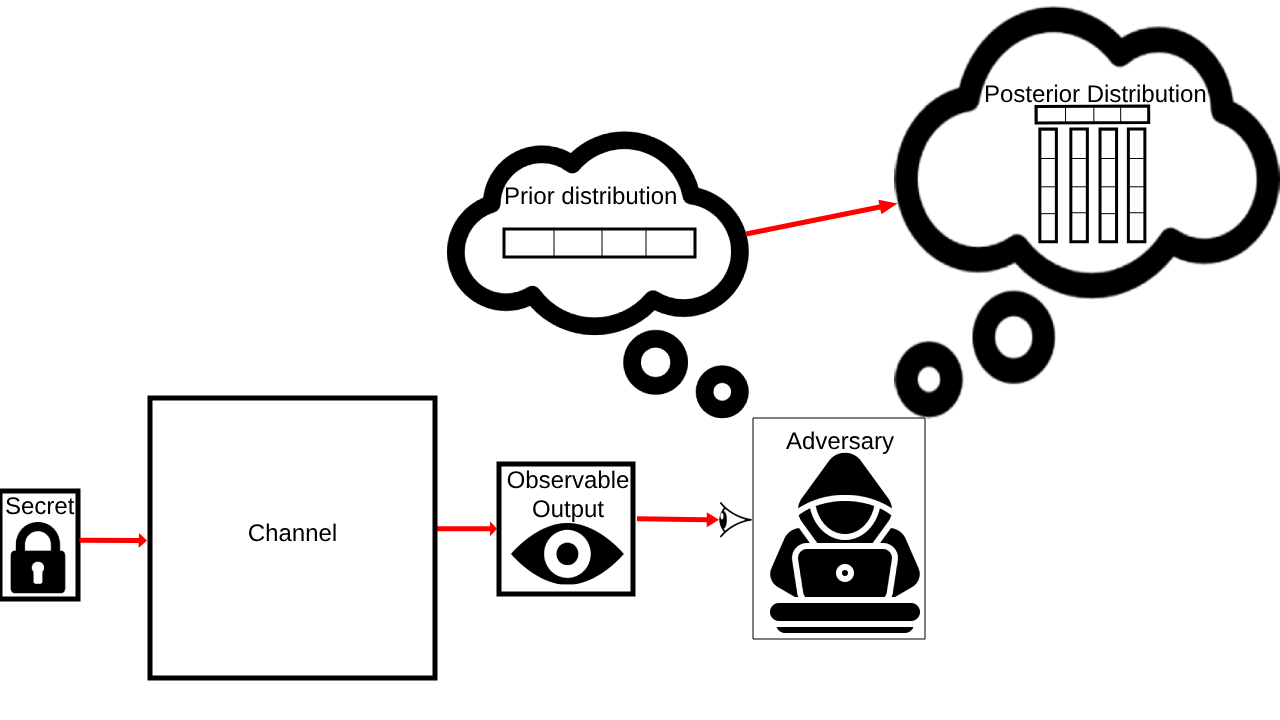
\includegraphics[width=\columnwidth]{channelAndFriends}
\caption{Figure representing the scenario we consider in Quantitative Information Flow.}\label{fig:channelAndFriends}
\end{figure}

We consider the $g$-vulnerability framework, introduced in (at the time of writing this work) main QIF textbook \cite{QIF}. This framework introduces new definitions, which we present more formally:

\begin{definition}[Gain Function]
A \emph{Gain Function} is a function $g : \mathcal{W} \times \mathcal{X} \rightarrow \mathbb{R}$, such that $g(w,x)$ defines the gain of the adversary if she takes the action $w$ when the secret value is actually $x$. 
\end{definition}

We do not have a loss for the system owner because we consider a zero-sum game: the gain of the adversary is exactly the loss of the people responsible for the system. 

\begin{definition}[Prior g-Vulnerability]
The \emph{Prior Vulnerability} of the system is defined as the average gain of the adversary if she takes the action that maximizes her expected gain, according to the distribution on secrets that represents her prior knowledge. Given a prior distribution on secrets $\pi$ and a gain function $g$, this is defined as:

$$V_g(\pi) = \max\limits_{w\in \mathcal{W}}\sum\limits_{x\in\mathcal{X}} \pi_x g(w,x)$$
\end{definition}

\begin{definition}[Posterior g-Vulnerability]
The \emph{Posterior Vulnerability} of the system is defined in the same way as the prior vulnerability, but considering the hyper-distribution that represents the posterior knowledge. Given a prior distribution on secrets $\pi$ and a channel $C$ and a gain function $g$, this is defined as:

$$V_g[\pi\triangleright C] = \sum\limits_{y \in \mathcal{Y}}\max\limits_{w\in \mathcal{W}}\sum\limits_{x\in\mathcal{X}} \pi_xC_{x,y} g(w,x)$$
\end{definition}

The posterior g-vulnerability represents what will be the expected gain of the adversary after the system runs, but the estimative is made according to the knowledge the adversary has before the system runs

\begin{definition}[Additive Leakage]
The \emph{Additive Leakage} can be defined as the difference between posterior and prior vulnerability:
$$\mathcal{L}_g^+(\pi,C) = V_g[\pi\triangleright C]-V_g(\pi)$$
\end{definition}

\begin{definition}[Multiplicative Leakage]
The \emph{Multiplicative Leakage} is the result of dividing the posterior vulnerability by the prior vulnerability values:
$$\mathcal{L}_g^\times(\pi,C) = \frac{V_g[\pi\triangleright C]}{V_g(\pi)}$$
\end{definition}

There are many valuable theoretical results about channels regarding the relationships between prior and posterior $g$-vulnerabilities. We mention some of these results:

\begin{enumerate}
\item The chapter 7 of the main QIF textbook at the time of this writing \cite[Chapter~7]{QIF} shows results about the \emph{capacity} of a channel, which is the maximum possible (additive or multiplicative) leakage that can happen through a channel if we fix either the prior, the gain function or neither.
\item Chapter 9 of the same book \cite[Chapter~9]{QIF} shows results about \emph{refinement} of channels: in short, a channel is strictly better (for all priors and gain functions) than another channel in respect to the posterior vulnerability if and only if it can be written as a post-processing of this other channel.
\item Chapter 10 of the same book \cite[Chapter~10]{QIF} presents the notion of \emph{Dalenious vulnerability}: it might be the case that the adversary is interested in a secret other than the one considered in the system, and can obtain information about this other system via a known joint distribution between this other secret and the secret that the system considers. In this case, a channel is also strictly better than another in respect to Dalenious leakage, for any such joint distribution and gain function, if and only it can be written as a post-processing of this other channel.
\item Finally, chapter 11 \cite[Chapter~11]{QIF} discusses the axiomatic characterization of the notion of vulnerability, and even how some results can be obtained by different axioms that consider the worst-case scenario instead of the average gains of the adversary.
\end{enumerate}

Even though most of the work on Quantitative Information Flow was developed with a stronger focus on measuring how system a system is, the $g$-vulnerability framework can be considered a general notion for quantifying information flow. This means that, in the future, we might be able to use it in the areas explored in this work, as some can be viewed in terms of information flows.

\subsection{Fairness $\times$ Privacy}

Some impossibility results in the literature argue why it is impossible to achieve both privacy and group fairness constraints under non-trivial accuracy \cite{Rachel}. We also have positive results that show how stasifying privacy constraints can help mitigate group unfairness \cite{makhlouf2024systematicformalstudyimpact}\cite{makhlouf2024impact}\cite{arcolezi2023local}, and we also have similar positive results results for individual fairness notions \cite{Awareness}.

\begin{enumerate}
	\item \qm{A systematic and formal study of the impact of local differential privacy on fairness: Preliminary results} \cite{makhlouf2024systematicformalstudyimpact} aims to provide theoretical results that relate how training a machine learning model on a dataset in which local differential privacy mechanisms were applied can impact the fairness of this model if the data-gatherer does not try to reverse the applied noise. The results are provided for a simplified machine learning model, from a theoretical perspective.
	\item \qm{On the impact of multi-dimensional local differential privacy on fairness} \cite{makhlouf2024impact} aims to evaluate experimentally how training a machine learning model on a multi-dimensional data set in which local differential privacy mechanisms were applied can impact the fairness of the model, again if the data-gatherer does not try to reverse the noise.
	\item \qm{(local) differential privacy has no disparate impact on fairness.} \cite{arcolezi2023local} executes an empirical evaluation of the impact of many Local Differential Privacy mechanisms on fairness when we do not try to reverse the applied noise, including a new privacy budget allocation scheme based on the domain size of sensitive attributes.
	\item \qm{Fairness through awareness} \cite{Awareness} introduces a notion of individual fairness that is a generalization of differential privacy and explores the relationship between this notion of fairness, differential privacy, and statistical disparity.
	\item \qm{On the compatibility of privacy and fairness} \cite{Rachel} presents theoretical results that show the impossibility of having a classifier that is not trivially accurate and at the same time satisfies $(\epsilon,0)$-differential privacy and equality of opportunity constraints. The paper also shows a PAC learner for an approximate fairness definition they provide.
	\item \qm{Exploring fairness and privacy in machine learning} \cite{henao2023exploring} compiles results that relate the concepts of privacy and fairness, and also causal discovery.
	\item \qm{Toward learning trustworthily from data combining privacy, fairness, and explainability: an application to face recognition} \cite{franco2021toward} discusses the use of Homomorphic Encryption in combination with fair representation learning \cite{zemel2013learning} to provide both privacy and fairness guarantees, respectively, when training machine learning models. Then the paper discusses how to provide local and global explanations for the model.
\end{enumerate}


\subsection{Fairness $\times$ QIF}
% Falar que nao vamos explorar essa aqui, fica pro futuro

One possibility of measuring fairness with Quantitative Information Flow notions is to measure the \emph{reverse flow}: instead of looking at how much observing the output of a model helps in estimating input values (this would be a privacy concern), we measure how much observing the sensitive attribute helps in estimating output values. This idea is already explored in previous works \cite{Bruno}\cite{nogueira2023relation}, so we won't explore it in this work.

\subsection{Privacy $\times$ QIF}

As QIF aims to quantify the flow of information, we can naturally consider applying it to the privacy scenario, by measuring how much information leaks about an arbitrary individual. One general idea is that differential privacy is a worst-case notion and $g$-vulnerability is an average-case notion, and there are results \cite{QIF} showing that differential privacy implies bounds on leakage under arbitrary gain functions and prior distributions, but not the opposite.

\begin{enumerate}
	\item \qm{On the information leakage of differentially-private mechanisms} \cite{alvim2015information} discusses the relations between differential privacy and $g$-vulnerability, including bounds on $g$-leakage as a function of the $\epsilon$ parameter of differential privacy, and the fact that there is no bound on differential privacy as a function of the $g$-vulnerability.
	\item \qm{Explaining epsilon in local differential privacy through the lens of quantitative information flow} \cite{fernandes2022explaining} discusses how the $\epsilon$ parameter of Differential Privacy is related to max-case $g$-vulnerability: $e^\epsilon$ is exactly the multiplicative max-case channel capacity under a fixed prior. This work also discusses many other theoretical results relating $g$-vulnerability notions with differential privacy.
\end{enumerate}

\section{Contributions}
Besides the literature review, this work has three main theoretical contributions, which we cover in the three subsections of this section:

\begin{enumerate}
	\item We identify qualitative questions about the premises of recent papers on the impact of Local Differential Privacy obfuscation mechanisms on fairness metrics, and thus questioning the conclusions obtained.
	\item We analize the possibility of distributing noise among variables with different degrees of sensibility for the reduction of the total noise in Local Differential Privacy obfuscation mechanisms, and conclude that this is not a good idea for various reasons we discuss in the second subsection of this section.
	\item We try a new approach, inspired on a recent paper \cite{fernandes2022explaining} that models the $\epsilon$ parameter of $\epsilon$-LDP, to modeling the $\delta$ parameter of $(\epsilon, \delta)$-LDP within the QIF framework, and conclude that it is not possible to do with this approach.
\end{enumerate}

\subsection{The impact of Local Differential Privacy mechanisms on fairness metrics}\label{subsec:ldpunfair}

{\color{red} Eu acho que tem isso salvo em algum lugar no computador. Lembrar da questao do Ramon de que o modelo treinado no dado com ruido nao tem problema porque ele vai ser usado em dados sem ruido estando pronto de qualquer forma.}

{\color{red} \begin{enumerate}
	\item Aplicar ruido em uma soh variavel dah problemas de privacidade, porque a menos que confiemos totalmente no coletor de dados (e nesse caso nao compensa aplicar ruido nenhum), ele pode reverter o ruido e usar um modelo treinado com a distribuicao sem ruido para inferir o valor da variavel sensivel a partir das outras. A terceira parte dessa secao de contribuicoes fala qual o problema em aplicar soh na variavel sensivel e nas correlacionadas.
	\item Mesmo no caso de aplicar ruido em todas as variaveis, nao faz sentido confiar que o coletor de dados nao vai reverter o ruido e treinar um modelo injusto.
	\item Mesmo que confiemos totalmente no coletor para nao reverter o ruido e aplicamos ruido em todas as variaveis para fins de privacidade, ele nao reverter so limita as opcoes que ele tem de trade-off entre fairness e acuracia.
\end{enumerate}}

\subsection{How to distribute the Local Differential Privacy budget between variables with varying levels of importance}\label{subsec:ldpbudget}

One simple mechanism to satisfy the Local Differential Privacy constraints of Definition \ref{def:epsilonLDP} is \textbf{Randomized Response}, described in \ref{def:nrr}.

\begin{definition}[n-Randomized Response]\label{def:nrr} Let $|\mathcal{X}| = n$. Then, the Randomized Response Mechanism $\mathcal{K}$ that maps from $\mathcal{X}$ to $\mathcal{X}$ can be defined as:
	\[
	\mathcal{K}(x) = 
	\begin{dcases*}
		x
		& with probability $\frac{e^\epsilon}{n-1+e^\epsilon}$\,, \\[1ex]
		y 
	   	& with probability $\frac{1}{n-1+e^\epsilon}$\,.
	\end{dcases*}
	\]
For any values $x\neq y$ such that $x,y\in\mathcal{X}$.
\end{definition}

Notice that this adds up to one: $\frac{e^\epsilon}{n-1+e^\epsilon}+(n-1)\frac{1}{n-1+e^\epsilon}=1$. Also, this mechanism satisifies the $\epsilon-LDP$ restriction from Definition \ref{def:epsilonLDP}, as we show in Lemma \ref{lem:rrldp}.

\begin{lemma}\label{rrldp} n-Randomized Response (Definition \ref{def:nrr}) satisifes $\epsilon-LDP$ (Definition \ref{def:epsilonLDP}).
\end{lemma}
\begin{proof}
	Let $S$ be any subset of the set of all outputs of $\mathcal{K}$. Notice that, by the definition of $\mathcal{K}$, this is a subset of secrets. Also, let $x \in \mathcal{X}$ and $\epsilon > 0$.
	If $x\in S$, then $P(\mathcal{K}(x) \in S) = \frac{|S|-1+e^\epsilon}{n-1+e^\epsilon}$, otherwise $P(\mathcal{K}(x) \in S) = \frac{|S|}{n-1+e^\epsilon}$.
	Now let $x,x' \in \mathcal{X}$ be any pair of secrets. We will divide the proof into five parts:
	\begin{enumerate}
		\item If $S = \emptyset$, then $P(\mathcal{K}(x) \in S) = P(\mathcal{K}(x') \in S) = 0$, so trivially $P(\mathcal{K}(x) \in S) \leq e^\epsilon P(\mathcal{K}(x')$.
		\item If $x\in S$, $x'\in S$, then $P(\mathcal{K}(x) \in S) = \frac{|S|-1+e^\epsilon}{n-1+e^\epsilon} \leq e^\epsilon \frac{|S|-1+e^\epsilon}{n-1+e^\epsilon} = e^\epsilon P(\mathcal{K}(x')\in S)$, as $e^\epsilon > 1$ when $\epsilon > 0$.
		\item If $x\in S$, $x'\notin S$, then $P(\mathcal{K}(x) \in S) = \frac{|S|-1+e^\epsilon}{n-1+e^\epsilon} = e^\epsilon\frac{\frac{|S|-1}{e^\epsilon}+1}{n-1+e^\epsilon} \leq e^\epsilon\frac{|S|-1+1}{n-1+e^\epsilon} = e^\epsilon \frac{|S|}{n-1+e^\epsilon} = e^\epsilon P(\mathcal{K}(x')\notin S)$, as $e^\epsilon > 1$ when $\epsilon > 0$.
		\item If $x\notin S$, $x'\in S$, then $P(\mathcal{K}(x) \notin S) = \frac{|S|}{n-1+e^\epsilon} \leq \frac{|S|-1+e^\epsilon}{n-1+e^\epsilon} \leq e^\epsilon \frac{|S|-1+e^\epsilon}{n-1+e^\epsilon} = e^\epsilon P(\mathcal{K}(x')\in S)$.
		\item If $x\notin S$, $x'\notin S$, then $P(\mathcal{K}(x) \notin S) = \frac{|S|}{n-1+e^\epsilon} \leq e^\epsilon \frac{|S|}{n-1+e^\epsilon} = e^\epsilon P(\mathcal{K}(x')\notin S)$, as $e^\epsilon > 1$ when $\epsilon > 0$.
	\end{enumerate}
\end{proof}

Notice that all probabilities are inversely proportional to $n$, but $n$ increases exponentially in respect to the number of variables for each data point. This means that in real applications with many attributes, the probabilities might get prohibitively small. Inevitably this leads to exponentially more data being necessary to reach statistically significant conclusions about it when we increase the number of variables collected per data point. One possible solution to this is obfuscating only the privacy-sensitive variables. For instance, in the scenario described at Figure \ref{fig:sensitiveVars}, most people would be satisfied with obfuscating only {\color{red} X} out of {\color{red} Y} variables.

{\color{red} BOTAR FIGURA}

{\color{red} Problema de estar correlacionado com outros dados, entao daria pra usar eles pra inferir os dados sensiveis.}

{\color{red} Essa correlacao pode ser descoberta de outras bases de dados inclusive, e mesmo que nao revelasse nada sobre o sensivel A, poderia usar um conjunto E de atributos pra inferir o sensivel, e descobrir informacao sobre a relacao entre A e X que nao se sabia ser correlacionado com o A. Ou seja, na filosofia de QIF ainda e ruim porque esta adicionando informacao em relacao ao que se tinha antes de informacao.}

{\color{red} Alem disso temos a necessidade de ter os dados sensíveis pra conseguir medir o quao injusto esta sendo o algoritmo final, possivelmente ate mesmo pra motivos legais.}

{\color{red} Definicao razoavel pro caso em que so importa os atributos sensiveis, formalizacao mesmo}

{\color{red} Como a distribuicao eh desconhecida para a pessoa que esta aplicando o ruido (se nao fosse desconhecida nao tem porque nem ela enviar o dado, melhor enviar a distribuicao toda), entao o mecanismo teria que funcionar em qualquer distribuicao. Citar o exemplo de distribuicao em que nao vai funcionar, e que a principio nao daria pra saber o quao correlacionado eh porque nao temos os dados.}

\subsection{Modeling the $\delta$ parameter of $(\epsilon,\delta)$-LDP within the Quantitative Information Flow framework}\label{subsec:ldeltap}

{\color{red} Esse tem nos papeis, e basicamente nao funcionou ate onde tentei.}

{\color{red} A ideia eh que max-QIF pega o pior caso com probabilidade maior que 0, e epsilon-LDP aceita zero chance de falha. max-delta-LDP pega o pior caso com probabilidade maior que delta, e delta-epsilon-LDP aceita delta chance de falha, entao talvez daria pra botar um bound usando delta-max-QIF.}

{\color{red} Tiveram mais tentativas, mas a linha principal foi primeiro ver o que o teorema do paper da Natasha significa em termos logicos (para todo epsilon e canal, etc.), e tentar provar trocando o axioma de max-QIF para max-delta-QIF, e ver se o mesmo bound com $\mathcal{M}Lift(C)$ funciona. No final das contas, eu acredito que mostrei que o bound, da forma como foi dado, eh equivalente a uma igualdade de outros termos, e provei que vai existir um canal constante que faz o bound nao funcionar.}

\section{Conclusions}

We can summarize the results obtained as following:

\begin{enumerate}
	\item There are some problems
	\item
	\item
\end{enumerate}

\bibliographystyle{IEEEtran}
\bibliography{IEEEexample}

\end{document}
